\section{Auswertung}
\label{sec:Auswertung}
\subsection{Messung der Kennlinie des Geiger-Müller Zählrohrs}
In Tabelle \ref{tab:Kennlinie} ist die Anzahl, der in dem Geiger-Müller gemessenen Impulse innerhalb von einer Minute abhängig von der Spannung aufgeführt. 

\begin{table}[http]
  \centering
  \caption{Aufgeführt ist die Anzahl der gemessenen Impulse $n$ abhängig von der eingestellten Spannung $U$.}
  \label{tab:Kennlinie}
  \sisetup{table-format=1.1, per-mode=reciprocal}
  \begin{minipage}[t]{0.4\textwidth}
  \begin{adjustwidth}{3cm}{}
    \begin{tblr}[t]{
      colspec = {S[table-format=3.0] S[table-format=5.0]},
      row{1} = {guard, mode=math},
    }
    \toprule
    U \mathbin{/} \unit{\volt} & n  \\
    \midrule
    300  &       0 \\
    320  &       0 \\
    340  &   15764 \\
    360  &   16310 \\
    380  &   16283 \\
    400  &   16605 \\
    420  &   16335 \\
    440  &   16456 \\
    460  &   16496 \\
    480  &   16630 \\
    500  &   16813 \\
    520  &   17344 \\

    \bottomrule
    \end{tblr}
  \end{adjustwidth}{}{} 
\end{minipage}
\hfill
\begin{minipage}[t]{0.4\textwidth}
  \begin{adjustwidth}{-1.5cm}{}
  \begin{tblr}[t]{
      colspec = {S[table-format=3.0] S[table-format=5.0]},
      row{1} = {guard, mode=math},
    }
    \toprule
    U \mathbin{/} \unit{\volt} & n  \\
    \midrule
    540  &   16841 \\
    560  &   17499 \\
    580  &   16949 \\
    600  &   16819 \\
    620  &   16935 \\
    640  &   16965 \\
    660  &   17058 \\
    680  &   17225 \\
    700  &   17472 \\
    720  &   17941 \\
    740  &   18995 \\
    760  &   20291 \\
    \bottomrule
  \end{tblr}
  \end{adjustwidth}
\end{minipage}
\end{table}
Damit kann die Kennlinie bestimmt werden.
Von $n$ wird der Logaritmus gebildet und gegen $U$ aufgetragen.
Daraus ergibt sich der in Abbildung \ref{fig:plot} gezeigte Verlauf.
Es wird eine lineare Regression durchgeführt, bei der die letzten drei Werte aus der Tabelle vernachlässigt werden.
Grund dafür ist, dass sich diesem Abschnitt die Abstände zwischen den Werten stark vergrößern, und diese Werte damit zum Bereich der Dauerentladung gehören.

\begin{figure}[H]
  \centering
  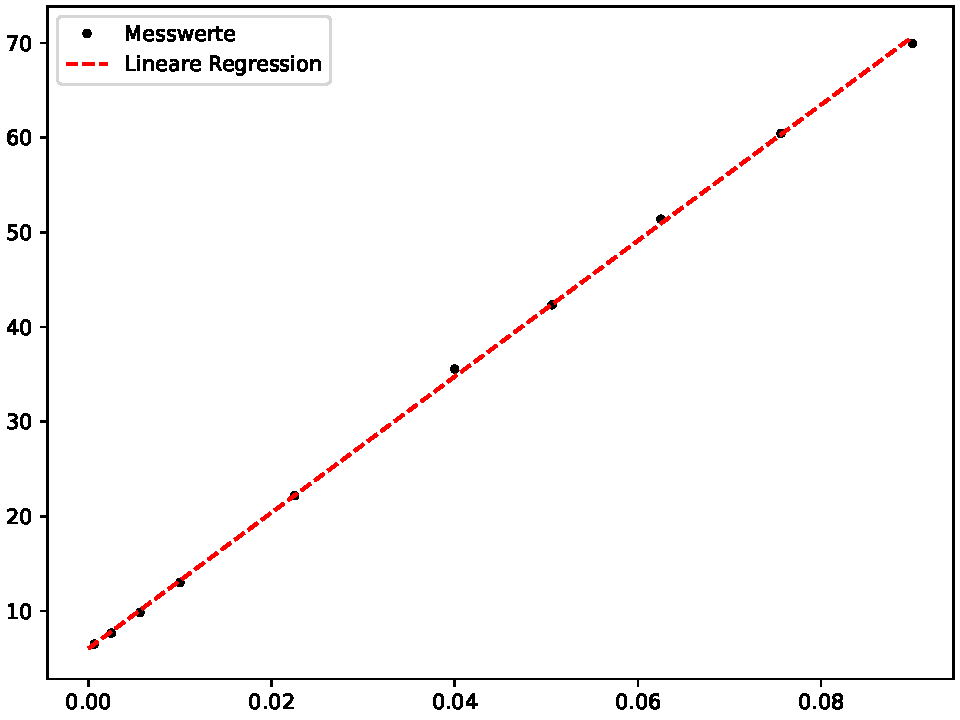
\includegraphics{plot.pdf}
  \caption{Abgebildet ist der Logaritmus der gemessenen Impulse in Abhängigkeit zur Spannung.}
  \label{fig:plot}
\end{figure}
\noindent Die Steigung dieser Ausgleichsgeraden ist die relative Zählrate mit $\frac{\increment N}{N}=\qty{1.9904(0.3183)e-04}{_}$.
Damit ist nach Gleichung \ref{eqn:relativ} die Steigung $s=\qty{1.9904(0.3183)e-04}{\percent\per\volt}$.

\subsection{Bestimmung der Totzeit}
Aus der Bestimmung der Totzeit mit dem Oszilloskop ergibt sich ein Wert von $\tau_{1}=\qty{250(25)}{\micro\second}$.
Für die Bestimmung mithilfe der zwei-Quellen Methode wurde die Anzahl der Zerfälle in zwei Minuten bei zwei Beta-minus Strahlern gemessen.
Für den Ersten ergibt sich $n_1=158675$.
Bei dem zweiten Strahler wird sich $n_2=142577$ gemessen und für beide zusammen $n_{12}=264863$ Zerfälle in zwei Minuten.
Daraus folgen die Zählraten $N_1=\qty{1322.2917}{\per\second}$, $N_2=\qty{1188.1417}{\per\second}$ und $N_{12}=\qty{2207.1917}{\per\second}$.
Durch Einsetzen in Formel \ref{eqn:totzeit} wird die Totzeit berechnet.
Der resultierende Wert entspricht $\tau_{2}=\qty{96.508}{\micro\second}$.